\section{将内存映射到文件进行流式处理}

上一章讨论了 CUDA kernel 如何作为纯函数式构件嵌入良构系统：kernel 只处理矩阵、配置和数值结果，
而不应认识文件、路径或用户接口。本章沿着这条边界继续向外走，讨论矩阵如何进入和离开系统。
对于端到端 SVD 程序，矩阵如何被验证、如何被转换为主机侧连续内存、如何被输出到下游工具，同样会影响可扩展性
（scalability）、可复现性（reproducibility）与故障语义（failure semantics）。

本章聚焦 \texttt{io.cpp}。它不是算法层的附属脚本，而是整个系统的数据平面（data plane）：
它定义了矩阵流的外部格式、跨平台字节序、文件映射生命周期、读写游标、文本兼容格式以及
policy-based stream 抽象；最新实现还增加了面向计算派发的单游标读取器（single-cursor dispatch reader）
与页锁定主机任务缓冲区（pinned host task buffer）。若说 \texttt{kernels.cu} 处理“如何计算”，那么 \texttt{io.cpp}
处理“什么数据以何种契约进入计算”。在 systems 视角下，这两者同等重要；因为任何计算内核最终都只能处理
已经被正确表示、正确边界化、正确拥有的数据。

\subsection{设计目标：把 I/O 从批量文件操作重构为矩阵流}

\texttt{io.cpp} 的首要目标不是提供一个简单的 \texttt{read()} / \texttt{write()} 包装，而是把文件视为
矩阵序列（matrix stream）。外部文件中可以顺序存放多张矩阵，应用层逐张读取、逐张计算、逐张写回。
这种接口具有三个系统层面的意义。

\paragraph{第一，降低应用层驻留压力。}
若接口强迫调用者一次性读取完整文件，应用层就必须同时持有所有测试矩阵、所有中间结果或所有输出。
对于 SVD 这类输出规模接近输入规模的算法，批量驻留很快会放大为
\[
    O\left(\sum_i m_i n_i\right)
\]
级别的长期内存占用。流式接口把边界收缩到“当前矩阵”：
\[
    \texttt{read\_one} \rightarrow \texttt{compute} \rightarrow \texttt{write\_one}.
\]
这为下一章的生产者-消费者（producer-consumer）pipeline 提供了自然接口。

\paragraph{第二，稳定文件格式契约。}
二进制 \texttt{*.mat} 格式采用“头部 + 载荷”的重复结构：
\[
    (\texttt{rows},\texttt{columns},\texttt{payload})^*.
\]
其中头部由两个 \texttt{uint64\_t} 组成，载荷为 $rows\cdot columns$ 个 \texttt{double}。
每个矩阵都是自描述记录（self-describing record）：读取端不依赖外部索引表，也不需要先扫描全文件才能定位下一张矩阵。
这使 EOF、截断、维度溢出和载荷不足都可以在局部被发现。

\paragraph{第三，分离“流控制”与“序列化策略”。}
同一个 \texttt{MatrixInputStream<Policy>} 可以服务于二进制 \texttt{MatFilePolicy}，
也可以服务于文本 \texttt{TxtFilePolicy}。模板层只关心打开、读取下一张矩阵、写入下一张矩阵和刷新；
具体格式如何编码字节、如何解析数字、是否使用内存映射，都被下沉到 policy。这是 policy-based design
的价值：把稳定控制流放在模板里，把易变格式细节放在策略里。

\subsection{数据模型与文件格式}

I/O 层的核心领域对象是 \texttt{Matrix}：
\[
    \texttt{Matrix}=(rows,columns,values).
\]
\texttt{values} 使用行主序（row-major order）的一维 \texttt{std::vector<double>}。
这与主机侧 C++ 容器、文本输出顺序以及 GPU 入口前的数据准备保持一致。矩阵元素索引为
\[
    index(i,j)=i\cdot columns+j.
\]

二进制 \texttt{*.mat} 文件的单条记录可抽象为：
\[
    \begin{aligned}
        R ={} &
        \underbrace{
            \texttt{uint64\_be}(rows)\;\Vert\;\texttt{uint64\_be}(columns)
        }_{\text{metadata}}
        \;\Vert                                                         \\
              & \underbrace{
                    \texttt{float64\_be}(a_{00})\;\Vert\;\cdots\;\Vert\;
                    \texttt{float64\_be}(a_{m-1,n-1})
                }_{\text{payload}} .
    \end{aligned}
\]
其中 \texttt{\_be} 表示大端序（big-endian），也就是网络字节序（network byte order）。
文件整体为
\[
    F=R_0\Vert R_1\Vert\cdots\Vert R_{k-1}.
\]

这一格式选择体现了一个保守但重要的系统设计原则：磁盘格式应当独立于主机 ABI。
如果直接把主机内存中的 \texttt{double} 与 \texttt{size\_t} 原样写出，文件就会隐式依赖平台端序、
\texttt{size\_t} 宽度、结构体填充与浮点表示。当前实现至少显式固定了两个维度：

\begin{itemize}
    \item 维度字段固定为 $64$ 位无符号整数，而不是平台相关的 \texttt{size\_t}；
    \item 所有 $64$ 位模式在磁盘上使用网络字节序，读取时再转换回主机字节序。
\end{itemize}

代码中 \texttt{to\_network\_u64} 与 \texttt{from\_network\_u64} 通过 \texttt{std::endian}
判断本机端序，并在小端机器上执行字节交换（byte swap）。\texttt{double} 则先通过
\texttt{std::bit\_cast<std::uint64\_t>} 转换为 $64$ 位模式，再复用同一套端序逻辑。
这比手写按字节拼接更直接，也避免了违反严格别名规则（strict aliasing rule）。

需要诚实指出的是：当前格式隐含假设 \texttt{double} 采用 $64$ 位 IEEE 754 binary64 表示。
这是现代 x86-64、AArch64 与 CUDA 主机环境中的现实假设，但若要把 \texttt{*.mat} 提升为长期归档格式，
文件头中还应加入 magic number、format version、element type 与校验信息。本项目当前阶段选择最小头部，
是为了降低实现复杂度并保持测试数据可直接检查。

\subsection{内存映射：把文件访问交给虚拟内存系统}

\texttt{MatFilePolicy} 的二进制路径使用内存映射文件（memory-mapped file）。
平台相关的系统调用被限制在匿名命名空间内部：

\begin{table}[htbp]
    \centering
    \begin{tabular}{lll}
        \toprule
        职责    & POSIX                           & Windows                                             \\
        \midrule
        打开文件  & \texttt{open}, \texttt{fstat}   & \texttt{CreateFileW}                                \\
        建立映射  & \texttt{mmap}                   & \texttt{CreateFileMappingW}, \texttt{MapViewOfFile} \\
        释放与刷新 & \texttt{munmap}, \texttt{msync} & \texttt{UnmapViewOfFile}, \texttt{FlushViewOfFile}  \\
        调整大小  & \texttt{ftruncate}              & \texttt{SetEndOfFile}                               \\
        \bottomrule
    \end{tabular}
\end{table}

\begin{center}
    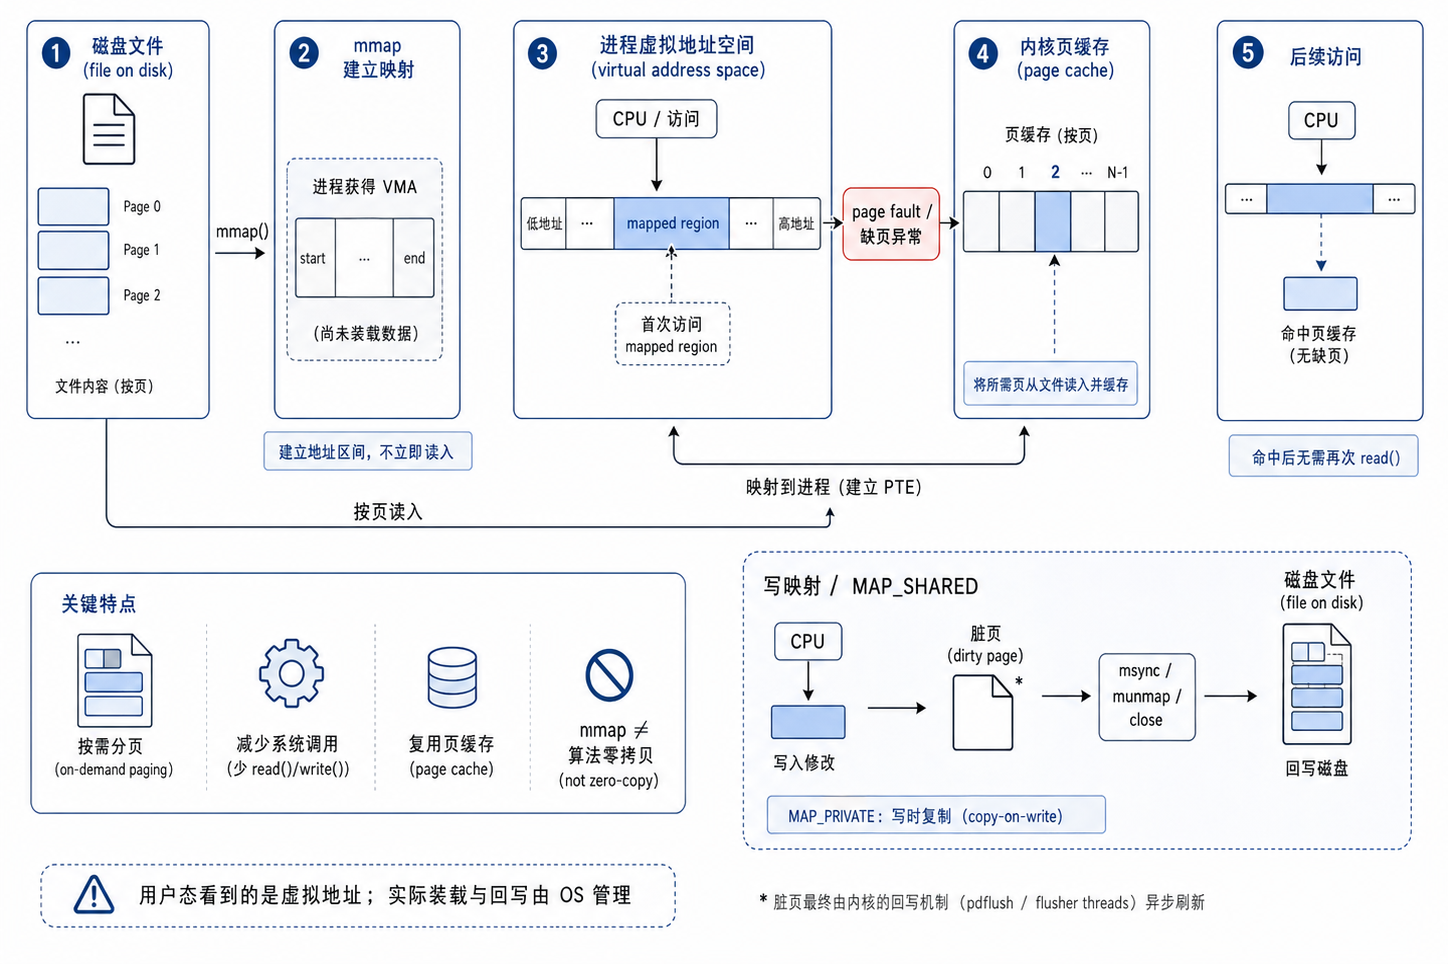
\includegraphics[width=0.92\textwidth]{figures/what-is-memory-mapping.png}
\end{center}

内存映射的系统语义可以概括为：
\[
    \text{file bytes}
    \longleftrightarrow
    \text{kernel page cache}
    \longleftrightarrow
    \text{process virtual address space}.
\]

程序不再围绕 \texttt{read()} 系统调用显式搬运固定大小缓冲区，而是获得一段虚拟地址范围。
实际页面在访问时由页错误（page fault）按需载入，并由操作系统的页缓存（page cache）管理复用与回写。
这通常减少了用户态缓冲区管理、系统调用频率与重复拷贝，但它并不等于算法层面的“零拷贝”。
当前实现仍然需要把磁盘上的网络序字节解码为主机侧 \texttt{std::vector<double>}，因为后续 CUDA 计算需要
连续、可拥有、可传输到设备的数值数组。


\subsection{只读映射：不可变字节视图与游标推进}

\texttt{MemoryMappedInputFile} 是二进制输入路径的资源拥有者。构造时，它完成三件事：

\begin{enumerate}
    \item 打开文件并查询文件长度；
    \item 若文件非空，则建立只读映射；
    \item 暴露 \texttt{std::span<const std::byte>} 作为不可变字节视图。
\end{enumerate}

析构时，它释放映射视图与底层文件句柄。拷贝构造和拷贝赋值被删除，移动构造和移动赋值被允许。
这与前一章中 \texttt{DeviceMatrix} 的思想一致：系统资源必须有唯一所有者（unique owner），
而不是被多个 C++ 对象模糊共享。这里的资源包括文件句柄、映射句柄和虚拟地址区间；任何一个被重复关闭，
都可能变成典型的 use-after-close 或 double-close 错误。

\texttt{MatReader::Impl} 在此基础上保存两个状态：
\[
    (\texttt{bytes},\texttt{cursor}).
\]
\texttt{cursor} 是当前读取位置。每次 \texttt{MatFilePolicy::read\_next} 执行时，状态转移为：
\[
    cursor
    \xrightarrow{\text{read header}}
    cursor + H
    \xrightarrow{\text{read payload}}
    cursor + H + 8mn,
\]
其中 $H=\texttt{sizeof(MatMetaData)}$。

读取路径的正确性由一组局部检查保护：

\begin{itemize}
    \item 若 \texttt{cursor == bytes.size()}，返回 EOF；
    \item 若剩余字节少于头部大小，报告截断头部（truncated header）；
    \item 将 \texttt{rows} 与 \texttt{columns} 从网络序转换为主机序；
    \item 检查维度是否超过本机 \texttt{size\_t}；
    \item 使用 checked arithmetic 计算元素数与载荷字节数；
    \item 若剩余字节少于载荷大小，报告截断载荷（truncated payload）。
\end{itemize}

这些检查看似朴素，但它们决定了文件格式能否被安全地暴露给系统其余部分。I/O 层不能把畸形输入
传递给 GPU kernel 后再期待 kernel “自然失败”。在系统边界处尽早拒绝坏数据，是降低故障半径
（blast radius）的基本做法。

\subsection{追加式输出映射：用容量管理替代频繁写系统调用}

输出路径由 \texttt{AppendMappedOutputFile} 管理。它把文件看作一个可增长的追加缓冲区：
\[
    (\texttt{data},\texttt{size},\texttt{capacity}).
\]
其中 \texttt{size} 是已经写入的逻辑字节数；\texttt{capacity} 是当前映射的物理文件容量。
每次追加新载荷时，代码先计算所需容量：
\[
    required=size+|payload|,
\]
若 \texttt{required <= capacity}，则直接 \texttt{memcpy} 到映射区尾部；否则按倍增策略扩容：
\[
    capacity'=\max(2^k\cdot capacity_0,required),
\]
其中初始容量下界为 $1\,\mathrm{MiB}$。

扩容过程是一个明确的四阶段协议：

\begin{enumerate}
    \item 刷新当前已写前缀；
    \item 取消当前映射；
    \item 调整底层文件大小到新容量；
    \item 重新建立写映射，并更新 \texttt{capacity}。
\end{enumerate}

析构时，\texttt{close()} 会尝试刷新已写前缀，释放映射，然后把文件截断到逻辑 \texttt{size}。
这一步很关键：倍增扩容会让底层文件暂时大于真实内容，最终必须恢复为精确长度，否则下游读取器会把尾部空洞
解释为额外记录或截断记录。

从摊还分析（amortized analysis）看，倍增扩容使 $N$ 字节输出的映射重建次数为
\[
    O(\log N),
\]
而普通追加写入路径为 $O(1)$。代价并没有消失：重映射会触发同步、取消映射和文件截断操作，
包括 \texttt{msync} / \texttt{FlushViewOfFile} 以及
\texttt{munmap} / \texttt{UnmapViewOfFile}。但相比每个小块都执行系统调用，它把高频路径压缩为
用户态内存拷贝，把低频路径交给容量管理。

\begin{center}
    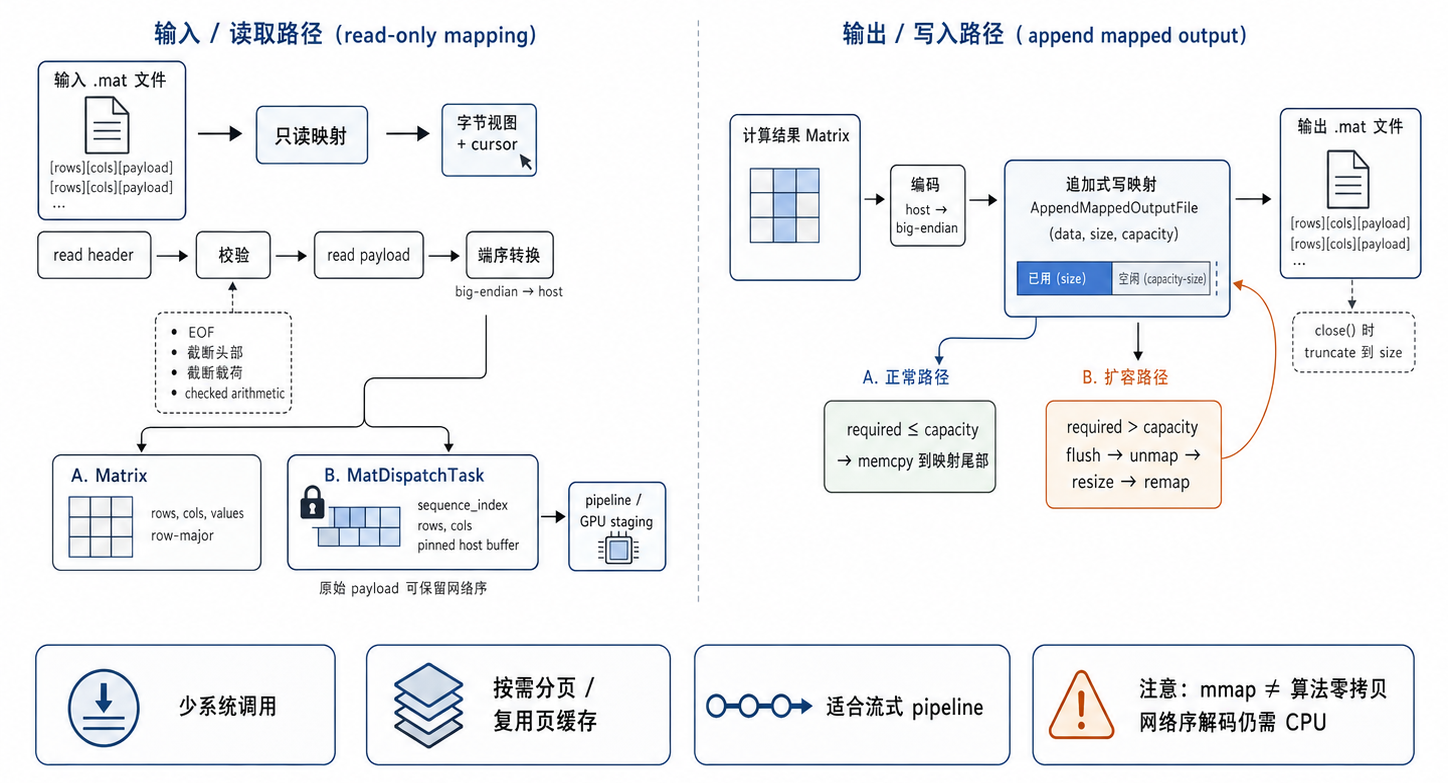
\includegraphics[width=0.92\textwidth]{figures/memory-mapping-rw.png}
\end{center}

\subsection{编码与解码：分块处理而不是整块临时复制}

二进制记录的载荷是 $rows\cdot columns$ 个 $64$ 位浮点模式。由于磁盘使用网络序，
读写都需要执行逐元素转换。当前实现采用固定大小分块：
\[
    B=32\cdot1024 \text{ elements}.
\]

读取时，\texttt{MatFilePolicy::read\_next} 直接从映射字节区按块取出 $64$ 位模式：
\[
    encoded_i \rightarrow \texttt{from\_network\_u64} \rightarrow \texttt{bit\_cast<double>}.
\]
每个元素通过 \texttt{std::memcpy} 取出，而不是把 \texttt{std::byte*} 强转为
\texttt{std::uint64\_t*}。这避免了未对齐访问（unaligned access）与别名规则风险。

写入时，\texttt{MatFilePolicy::write\_next} 先写网络序头部，再复用一个
\texttt{uint64\_t} 编码块向量。每个块完成：
\[
    double_i \rightarrow \texttt{bit\_cast<uint64\_t>} \rightarrow \texttt{to\_network\_u64}
    \rightarrow \texttt{append(bytes)}.
\]
这里的分块有两个作用。第一，它限制临时编码缓冲区大小，不随矩阵规模线性增长。
第二，它让输出路径可以连续追加多个字节块，而不需要为每张矩阵构造一个完整的编码副本。
因此，虽然 \texttt{Matrix} 本身仍然以完整矩阵为粒度进入计算，序列化层的额外空间为
\[
    O(B),
\]
而不是 $O(mn)$。

\subsection{派发读取：把字节流先送入页锁定任务缓冲}

上面的 \texttt{MatReader} 路径服务于传统矩阵流接口：
\[
    \texttt{*.mat\ bytes}
    \longrightarrow
    \texttt{Matrix}.
\]
新加入的 \texttt{MatDispatchReader} 则面向下一层 pipeline 的任务派发（task dispatch）场景。它不立即把载荷解码为
\texttt{std::vector<double>}，而是把单条 \texttt{*.mat} 记录拆成更接近调度单元的数据结构：
\[
    \texttt{MatDispatchTask}
    =
    (\texttt{sequence\_index},\texttt{rows},\texttt{columns},\texttt{buffer}).
\]
其中 \texttt{buffer} 是 \texttt{PinnedHostTaskBuffer}，底层通过 \texttt{cudaMallocHost} /
\texttt{cudaFreeHost} 管理一整块页锁定主机内存（page-locked host memory）。这条路径的核心思想不是替代
\texttt{MatInputStream}，而是给更高吞吐的生产者-消费者 pipeline 预留一个更合适的输入形态：主线程可以用一个
单调文件游标顺序读取记录，把原始网络序 payload 放进可复用的 pinned buffer，再把解析、计算或异步拷贝交给后续阶段。

\paragraph{数据结构上，特殊情况被折叠成普通区间。}
\texttt{PinnedHostTaskBuffer} 没有为输入区、解码区、GPU staging 区分别维护多块 allocation，
而是把它们表达为同一块连续 pinned memory 内的两个 span：
\[
    \underbrace{[0,\texttt{input\_bytes})}_{\text{raw payload}}
    \quad\Vert\quad
    \underbrace{[\texttt{input\_bytes},\texttt{input\_bytes}+\texttt{workspace\_bytes})}_{\text{workspace}}.
\]
调用者通过 \texttt{mutable\_input\_bytes()} 与 \texttt{mutable\_workspace\_bytes()} 获得两个视图。
这是一种很朴素的好品味：不是让每个阶段各自发明一套临时缓冲，而是在 I/O 边界把“输入字节”和“后续工作区”
统一成一个明确拥有者。移动构造和移动赋值只移动指针与大小，拷贝被删除；因此任务可以在线程队列中移动，
但不会意外复制 pinned memory。

\paragraph{容量策略上，复用比频繁分配更重要。}
\texttt{reserve(input\_bytes, workspace\_bytes)} 先计算总需求：
\[
    required = input\_bytes + workspace\_bytes.
\]
若已有容量足够，只更新输入区和工作区大小；若容量不足，则按倍增策略增长，初始下界为
$64\,\mathrm{KiB}$。因此同一个 \texttt{MatDispatchTask} 可以被读取循环反复复用：小矩阵不会导致频繁
\texttt{cudaMallocHost} / \texttt{cudaFreeHost}，大矩阵也只在超过历史峰值时触发重新分配。
这与输出映射的摊还思想一致，只是资源从“文件映射容量”变成了“页锁定主机容量”。

\paragraph{语义上，派发任务保存的是原始载荷而不是已解码矩阵。}
\texttt{MatDispatchReader::read\_next} 的状态转移为：
\[
    \begin{aligned}
        \text{read header}
         & \longrightarrow
        \text{validate dimensions}
        \longrightarrow
        \text{reserve pinned buffer} \\
         & \longrightarrow
        \text{read payload bytes}
        \longrightarrow
        \text{assign sequence index}.
    \end{aligned}
\]
载荷仍保持磁盘上的网络字节序。若后续阶段需要传统 \texttt{Matrix}，可以调用
\texttt{decode\_dispatch\_task\_matrix} 完成逐元素解码；若未来 kernel wrapper 支持直接从 pinned staging buffer
构造输入，则也可以在工作区中完成解码并与 host-device copy 更紧密地衔接。
这给 pipeline 留出了演化空间，而没有把 CUDA stream、device pointer 或 kernel 调度塞进 I/O 层。

这里必须保持一个清醒的边界：pinned memory 不是免费资源。页锁定内存不能被操作系统随意换出，过量使用会挤压系统分页能力，
甚至拖慢整机。于是 \texttt{PinnedHostTaskBuffer} 只能解决“当前任务如何更适合被派发”的问题，
不能替代有界队列（bounded queue）和背压（backpressure）。真正的内存上界仍然要由 pipeline 控制：
\[
    M_{\mathrm{pinned}}
    \le
    \sum_{t\in\mathrm{in\ flight}}
    \texttt{capacity\_bytes}(t).
\]
如果 in-flight 任务数无界，pinned buffer 再漂亮也会把系统拖入资源耗尽。因此这条新路径和下一章的生产者-消费者队列
是一组配套设计：I/O 层让单个任务适合高速派发，pipeline 层决定同时允许多少任务存在。

\subsection{Policy-based stream：把格式差异从控制流中剥离}

\texttt{io.hpp} 中定义了两个 concept：
\[
    \begin{aligned}
        \texttt{MatrixInputPolicy}  & =
        \{\texttt{Reader},\texttt{open\_reader},\texttt{read\_next}\}, \\
        \texttt{MatrixOutputPolicy} & =
        \{\texttt{Writer},\texttt{open\_writer},\texttt{write\_next},\texttt{flush}\}.
    \end{aligned}
\]
它们把“什么是合法矩阵输入策略/输出策略”表达为编译期契约（compile-time contract）。
模板类 \texttt{MatrixInputStream<Policy>} 与 \texttt{MatrixOutputStream<Policy>} 只依赖这一契约，
并不依赖具体文件格式。

这一层的状态机非常小：
\[
    \texttt{MatrixInputStream}
    =
    (\texttt{reader},\texttt{eof}),
\]
\[
    \texttt{MatrixOutputStream}
    =
    (\texttt{writer}).
\]
输入端的 \texttt{read\_one} 调用 policy 的 \texttt{read\_next}；若返回 \texttt{false}，
流进入 EOF 状态，后续读取直接返回 \texttt{false}。输出端的 \texttt{write\_one} 调用
\texttt{write\_next}，\texttt{write\_all} 则在循环后统一 \texttt{flush}。

这种结构的关键收益不是“模板很漂亮”，而是依赖方向正确：

\begin{quote}
    流控制依赖抽象 policy；格式实现依赖底层文件机制；应用层依赖流接口。反过来的依赖都不存在。
\end{quote}

因此，新增一种格式，例如压缩二进制格式或 NumPy \texttt{.npy} 子集，并不需要修改 pipeline 的控制流；
只需要提供满足 concept 的新 policy。这是 C++20 concept 在系统设计中的实际价值：
它把运行期协议错误提前为编译期接口错误。

\paragraph{二进制 \texttt{*.mat} policy：吞吐优先的主路径。}
\texttt{MatFilePolicy} 是这套抽象的“正常路径”。它把前面已经讨论过的内存映射、固定头部、
网络字节序编码和追加式输出统一封装到
\texttt{open\_reader} / \texttt{read\_next} / \texttt{open\_writer} / \texttt{write\_next} / \texttt{flush}
这组接口后面。于是对上层而言，\texttt{*.mat} 只是“一个满足 concept 的 policy”，
而不是一串散落在控制流里的特殊分支。

这件事的系统意义在于：高性能实现被局部化了。页缓存、映射重建、字节序转换、
分块编码这些复杂性都留在 \texttt{MatFilePolicy} 内部；\texttt{MatrixInputStream} /
\texttt{MatrixOutputStream} 仍然只维持一个极小状态机。换句话说，性能优化存在，但它不污染抽象边界。

\paragraph{文本 \texttt{*.txt} policy：可检查性优先的兼容路径。}
\texttt{TxtFilePolicy} 提供文本矩阵流。其格式约定是：行内元素用空格分隔，行之间用换行分隔，
矩阵之间用空行分隔。读取器逐行解析：

\begin{itemize}
    \item 连续空白行在矩阵开始前被忽略；
    \item 一旦进入矩阵，空白行表示当前矩阵结束；
    \item 非空行必须至少解析出一个浮点数；
    \item 同一矩阵内每行列数必须一致；
    \item 文件结束时，若当前正在读取矩阵，则返回最后一张矩阵。
\end{itemize}

文本路径使用 \texttt{std::locale::classic()}，避免本地化小数点或分隔符影响解析。
写入时使用 \texttt{std::numeric\_limits<double>::max\_digits10} 精度，以尽量保证二进制浮点值经十进制文本
输出再读入后可以 round-trip。

从性能角度看，文本路径显然不是高吞吐路径。它需要执行十进制解析、格式化和更多分支判断。
但它在系统中仍然有价值：测试样例可读、调试输出可检查、用户可以手写小矩阵输入。
因此，把它放进 policy 层的意义，不是把文本伪装成“和二进制一样快”，而是让
\texttt{*.txt} 也通过同一套流接口接入系统。这样，\texttt{*.mat} 面向吞吐与稳定格式，
\texttt{*.txt} 面向可观察性（observability）与开发便利；二者共享抽象，不共享性能假设。

\subsection{错误模型：在边界处失败，而不是在深处腐化}

\texttt{io.cpp} 的错误模型以异常（exception）报告不可恢复错误。这里的异常不是控制流装饰，
而是对系统边界失败的直接编码。典型错误包括：

\begin{table}[htbp]
    \centering
    \begin{tabular}{lll}
        \toprule
        错误类别        & 检测位置                                   & 系统含义             \\
        \midrule
        文件打开失败      & 构造 reader / writer                     & 外部资源不可用          \\
        文件长度非法      & 映射前                                    & 底层文件状态不满足前置条件    \\
        头部截断        & \texttt{read\_next}                    & 记录边界被破坏          \\
        载荷截断        & \texttt{read\_next}                    & 元数据与实际字节数不一致     \\
        维度溢出        & checked arithmetic                     & 输入会导致本机地址空间或容器越界 \\
        pinned 分配失败 & \texttt{PinnedHostTaskBuffer::reserve} & 主机侧 staging 资源不足 \\
        派发载荷截断      & \texttt{MatDispatchReader::read\_next} & 任务边界被破坏，不能进入计算队列 \\
        行列不一致       & 文本解析                                   & 文本矩阵不是矩形结构       \\
        刷新失败        & \texttt{flush}                         & 输出持久化状态未知        \\
        \bottomrule
    \end{tabular}
\end{table}

特别值得注意的是 checked arithmetic。矩阵载荷大小由
\[
    bytes = rows\cdot columns\cdot 8
\]
决定。若这个乘法在 \texttt{size\_t} 中溢出，后续检查会得到一个错误的小值，进而可能接受畸形文件。
\texttt{checked\_multiply} 与 \texttt{checked\_add} 把这种风险变成显式异常。
这是一种很“朴素”的代码，但在系统边界上非常有品味：不要让整数溢出把坏输入伪装成好输入。

\subsection{性能模型：mmap 优化的是数据通路，而不是算法复杂度}

设某张矩阵有 $m$ 行、$n$ 列。二进制读取的主要 CPU 工作为：
\[
    O(mn)
\]
次 $64$ 位载荷解码和一次 $O(1)$ 头部解析。写入类似，为 $O(mn)$ 次编码和追加。
内存映射不改变这一渐近复杂度；它改变的是常数项、系统调用结构与缓存行为。

与显式 \texttt{read()} 循环相比，mmap 路径具有几个潜在优势：

\begin{itemize}
    \item 顺序扫描映射区时，操作系统可以执行预读（read-ahead）并复用页缓存；
    \item 应用层不需要管理输入缓冲区生命周期；
    \item 多个进程读取同一文件时，页缓存可以共享底层物理页；
    \item 输出追加的高频路径退化为对映射区的 \texttt{memcpy}。
    \item 派发读取路径可以把原始 payload 放入 pinned buffer，为后续异步 host-device copy 提供必要前提。
\end{itemize}

但同样存在代价：

\begin{itemize}
    \item 首次访问页面会产生 minor 或 major page fault；
    \item 大文件映射会消耗虚拟地址空间，尤其在地址空间受限平台上需要谨慎；
    \item 输出扩容需要解除映射、调整文件大小并重新映射；
    \item \texttt{msync} 或 \texttt{FlushViewOfFile} 的同步语义可能成为尾部延迟来源；
    \item 网络序转换仍然是 CPU 上的逐元素循环，不能被 mmap 自动消除。
    \item pinned memory 会降低操作系统调页自由度，必须通过任务复用和有界 in-flight 数量控制总量。
\end{itemize}

因此，本章的结论不应是“mmap 总是更快”。更准确的说法是：
当前 I/O 层用 mmap 把文件访问纳入虚拟内存管理，使顺序二进制矩阵流获得较低的用户态管理复杂度；
实际吞吐仍取决于存储设备、页缓存命中率、矩阵规模、编码转换成本和 pipeline 是否能与 GPU 计算重叠。

\subsection{与计算 pipeline 的接口边界}

从端到端视角看，I/O 层向上提供的是一组非常小的语义：

\[
    \texttt{bool read\_one(Matrix\&)}
\]
\[
    \texttt{void write\_one(const Matrix\&)}
\]
\[
    \texttt{void flush()}
\]

这个接口刻意没有暴露 mmap、文件句柄、字节序或文本解析细节。应用层只看到矩阵对象与 EOF。
这种边界使 pipeline 可以关注自己的核心问题：如何把输入矩阵送入 CUDA SVD，如何把输出矩阵交给消费者线程，
如何在计算与写入之间建立背压（backpressure）。

新增的派发接口则更接近高性能 pipeline 的内部边界：
\[
    \texttt{bool read\_next(MatDispatchTask\&, workspace\_bytes)}
\]
\[
    \texttt{Matrix decode\_dispatch\_task\_matrix(const MatDispatchTask\&)}.
\]
它比 \texttt{read\_one(Matrix\&)} 暴露更多信息：记录序号、原始 payload、预留工作区与 pinned allocation。
这不是抽象泄漏，而是层间契约的有意细化。传统流接口适合“读出一张矩阵再计算”的简单路径；
派发接口适合“先把一条记录变成可移动任务，再由后续阶段决定何时解码、何时拷贝、何时计算”的流水线。
两者共同存在，使项目不必为了高性能路径破坏已有的兼容 API。

与此同时，I/O 层也没有越界承担 GPU 责任。它不会分配 device memory，不会启动 kernel，
不会管理 CUDA stream，也不会为了“优化”而把文件映射地址直接交给设备侧。这样的克制很重要：
文件格式、主机内存、设备内存、并发 pipeline 是不同抽象层。若把它们混在一个对象里，
短期看似减少了函数调用，长期会制造难以测试的生命周期耦合。

\subsection{当前实现的边界与可演化方向}

当前 \texttt{io.cpp} 已经建立了清晰的数据平面，但它仍有几个需要明确记录的边界。

\paragraph{第一，流式粒度是矩阵级，而不是元素级。}
\texttt{MatReader} 映射整个文件，\texttt{read\_next} 每次解码一整张矩阵到 \texttt{std::vector<double>}。
这对 dense SVD 是合理的，因为 GPU kernel 本身需要完整矩阵参与迭代。但若未来处理的是超大矩阵的分块算法，
I/O 层就需要提供 tile stream 或 block stream，而不是 matrix stream。

\paragraph{第二，文件头还不是长期稳定格式。}
当前 \texttt{*.mat} 没有 magic number、版本号、校验和、元素类型枚举或压缩标志。
这使格式极简，但也意味着错误文件可能只能通过截断或维度异常被发现。
若该格式要跨项目复用，建议将记录头扩展为：
\[
    \texttt{magic},\quad \texttt{version},\quad \texttt{dtype},\quad
    \texttt{rows},\quad \texttt{columns},\quad \texttt{payload\_bytes}.
\]

\paragraph{第三，输出映射扩容是同步路径。}
倍增策略把重映射次数降到对数级，但每次重映射仍然会刷新、取消映射、截断文件并重新映射。
若输出吞吐成为瓶颈，可以考虑两类优化：一是基于输入规模预估输出总大小并一次性预分配；
二是在 producer-consumer pipeline 中让写线程批量聚合结果，降低 flush 频率。

\paragraph{第四，文本路径强调可读性，不强调吞吐。}
\texttt{TxtFilePolicy} 对开发体验很有价值，但它不应被误认为高性能输入路径。
大规模实验应优先使用 \texttt{*.mat}；文本格式更适合小样例、单元测试和人工检查。

\paragraph{第五，派发读取路径目前只覆盖 \texttt{*.mat}。}
\texttt{MatDispatchReader} 是二进制格式的专用优化路径，因为它依赖固定大小头部与可直接计数的二进制 payload。
文本格式需要逐行解析和列数校验，不适合原样塞入同一种 dispatch task。若未来要对文本输入也做异步读取，
更合理的做法是先把文本解析成 \texttt{Matrix} 或独立的 parsed task，而不是扭曲 \texttt{MatDispatchTask}
去同时表达两种完全不同的载荷语义。

\paragraph{第六，pinned buffer 只是 host-device 重叠的前置条件。}
页锁定内存让异步拷贝更有意义，但它本身不会自动带来 CUDA stream 重叠。要真正实现
\[
    \text{read/decode}
    \parallel
    \text{host-device copy}
    \parallel
    \text{kernel}
    \parallel
    \text{write}
\]
还需要 kernel 层提供异步接口，并由 pipeline 明确管理 stream、事件与任务生命周期。
因此当前 \texttt{PinnedHostTaskBuffer} 应被理解为一块稳固地基，而不是完整的异步执行框架。

\paragraph{第七，端序被固定，浮点语义仍依赖现实平台。}
网络字节序解决了字节排列问题，但没有把 \texttt{double} 的语义完全自描述化。
在现代 HPC 环境中这通常足够；但若追求跨几十年的归档稳定性，文件格式应显式声明 IEEE 754 binary64。

\subsection{小结}

本章把 \texttt{io.cpp} 定位为系统的数据平面（data plane）：它不实现 SVD，不编排 pipeline，
也不管理 CUDA 资源，而是把外部持久化介质抽象为一个类型安全的矩阵流。围绕这一目标，
它同时承担四类边界职责：定义二进制 \texttt{*.mat} 与文本格式契约，使用内存映射文件
（Memory-Mapped Files）降低顺序访问的用户态管理成本，执行网络字节序与 \texttt{double} 载荷之间的编码转换，
并在文件损坏、维度非法、映射失败或写入失败时尽早停止。

从系统设计角度看，I/O 层的价值不在于“读写文件”这件小事本身，而在于它把脏世界关在边界外：
坏输入不能越过 I/O 边界，资源不能泄露或重复释放，格式变化不能污染 pipeline 控制流，
高吞吐路径也不能牺牲可验证性。这样，下一章的 pipeline 才能把输入流、CUDA SVD kernel 与输出流组合起来，
而不必理解字节序、mmap 生命周期或文本解析细节。

这正是数值系统中经常被低估的部分。GPU kernel 可以把浮点吞吐推到很高，但系统最终的可信度，
往往取决于这些更安静的边界代码：它们决定数据是否被正确解释，错误是否被及时停止，
以及未来的扩展是否还能保持清楚的依赖方向。
